\begin{abstract}
A broad-band colour sensor can order source colours consistently, with its temperature scale set by the colour calibration. Example APDS-9960 counts are corrected for dark offsets, normalized by the clear response and transformed using a provisional RGB-to-XYZ matrix before applying McCamy's cubic approximation. Interior-window means are 2548, 3935 and 6114 K for warm, intermediate and cool states, with within-window standard deviations of 25, 18 and 91 K. The matrix is traced to a TCS3414CS application note, linking the temperature conversion to the transfer of a sensor-specific spectral calibration. The analysis distinguishes repeatable numerical conversion from colorimetric accuracy and from the physical temperature of an emitting body.
\end{abstract}
\begin{IEEEkeywords}
Correlated colour temperature, spectral mismatch, RGB calibration, chromaticity, Planckian radiation.
\end{IEEEkeywords}

\section{Colour temperature requires a colour measurement}
Correlated colour temperature (CCT) relates a source's chromaticity to that of a Planckian radiator. It does not imply that the source itself is a blackbody. The CIE's terminology guidance emphasizes the restrictions that arise when a spectrum departs from Planckian radiation\cite{CIE2022TN013}. A narrow-band source and a thermal source can therefore require different descriptions even if a numerical conversion returns a plausible value in kelvin.

McCamy's explicit cubic provides an efficient approximation to the chromaticity--CCT relation\cite{McCamy1992}. Its input must first be a meaningful colorimetric coordinate. An RGB sensor supplies device-specific spectral integrals, whereas CIE XYZ coordinates are defined through standard colour-matching functions. Treating the two triples as interchangeable omits the most consequential calibration step.

This issue is concrete for the conversion considered here. Its matrix coefficients are identical to those in Smith's application note for the TAOS TCS3414CS\cite{Smith2009TAOSAN000517}. That note derives a transform for that sensor using reference sources and describes obtaining a new matrix for another calibration family. The APDS-9960 has its own filtered photodiodes and spectral response\cite{apds9960}. Transferring the numerical matrix to another sensor makes its spectral response part of the calibration.

\section{From counts to provisional chromaticity}
Figure~\ref{fig:colour-temperature-apparatus} separates the relative-light acquisition from the independent reference needed to calibrate a colour transform. A fixed aperture and source geometry help maintain a reproducible incident spectrum. Covered readings determine electronic offsets; a change in ambient illumination is a separate contribution because it also has a spectrum.

\begin{figure}[!htbp]
\centering
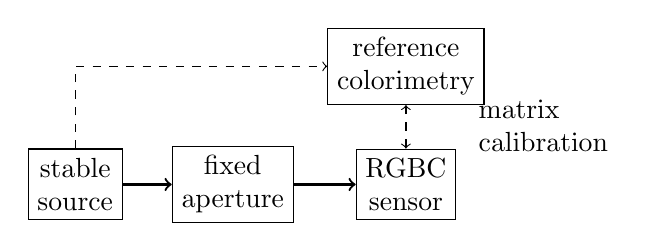
\begin{tikzpicture}[x=1cm,y=1cm]
 \node[draw,align=center] (s) at (.7,0) {stable\\source};
 \node[draw,align=center] (a) at (2.7,0) {fixed\\aperture};
 \node[draw,align=center] (d) at (4.9,0) {RGBC\\sensor};
 \node[draw,align=center] (r) at (4.9,1.5) {reference\\colorimetry};
 \draw[->,thick] (s)--(a);\draw[->,thick] (a)--(d);
 \draw[->,dashed] (s.north)--(.7,1.5)--(r.west);
 \draw[<->,dashed] (d.north)--(r.south);
 \node[right,align=left] at (5.7,.75) {matrix\\calibration};
\end{tikzpicture}
\caption{A relative sensor and independent colour reference view a reproducible source condition. A matrix fit requires several reference colours spanning the intended source family.}
\label{fig:colour-temperature-apparatus}
\end{figure}

For the example, the dark values are $D_C=3$, $D_R=D_G=2$ and $D_B=1$ counts. The normalized colour responses are $q_k=(C_k-D_k)/(C-D_C)$. They are transformed according to
\begin{equation}
 \begin{bmatrix}X\\Y\\Z\end{bmatrix}
 =\begin{bmatrix}
 -.14282&1.54924&-.95641\\
 -.32466&1.57837&-.73191\\
 -.68202&.77073&.56332
 \end{bmatrix}
 \begin{bmatrix}q_R\\q_G\\q_B\end{bmatrix}.
 \label{eq:colour-temperature-matrix}
\end{equation}
Here XYZ are provisional relative coordinates. Chromaticities are then $x=X/(X+Y+Z)$ \mbox{and $y=Y/(X+Y+Z)$}, subject to positive-domain checks. Because this matrix transformation is homogeneous, the common corrected-clear denominator cancels exactly in $x$ and $y$. The clear reading therefore contributes a working-range and validity check, rather than an independent chromaticity coordinate. This cancellation cannot correct an error in the spectral shape of the colour-channel response.

The adopted McCamy convention is
\begin{align}
 n&=\frac{x-.3320}{.1858-y},\\
 T_{\rm cp}/\mathrm{K}&=449n^3+3525n^2+6823.3n+5520.33.
 \label{eq:colour-temperature-cubic}
\end{align}
The positive cubic and linear coefficients are consistent with this denominator sign. Reversing the sign of the denominator requires reversing the odd-power terms. Values close to $y=.1858$, nonphysical coordinates and outputs outside the chosen 2000--10000 K screening interval are excluded. That numerical interval is a screen; it is not a calibrated accuracy specification or a test of distance from the Planckian locus.

\section{The example colour sequence}
The data pass from a warm state through an intermediate state to a cool state and return to warm. Four interior windows exclude transitions. Their chromaticity means move systematically from larger to smaller $x$ and $y$ across the three states. Returning to the initial colour brings both coordinates close to their earlier values.

\begin{figure}[!htbp]
\centering% Generated by prepare_drafts.py from the supplied CSV files.
\begin{tikzpicture}
\begin{groupplot}[group style={group size=1 by 2,vertical sep=1.15cm},
width=0.98\columnwidth,height=3.2cm,
grid=major,enlarge x limits=false,
legend style={font=\scriptsize,at={(0.5,1.03)},anchor=south,
legend columns=4,draw=none,fill=none,column sep=4pt},
title style={font=\scriptsize,at={(0.02,0.98)},anchor=north west,
fill=white,fill opacity=0.9,text opacity=1,inner sep=2pt},
ylabel style={font=\footnotesize},
xlabel style={font=\footnotesize},tick label style={font=\scriptsize}]
\nextgroupplot[ylabel={Indicative CCT (K)},title={(a) Provisional conversion}]
\addplot[csblue,solid,line width=0.8pt] table[col sep=comma,x=c0,y expr={(\thisrow{c18}-(0))*(1)}] {data/drafts/colour-temperature.csv};
\nextgroupplot[ylabel={Chromaticity (1)},xlabel={Device time (s)},title={(b) Matrix-derived chromaticities}]
\addplot[csblue,solid,line width=0.8pt] table[col sep=comma,x=c0,y expr={(\thisrow{c14}-(0))*(1)}] {data/drafts/colour-temperature.csv};
\addlegendentry{$x$}
\addplot[csred,dashed,line width=0.8pt] table[col sep=comma,x=c0,y expr={(\thisrow{c15}-(0))*(1)}] {data/drafts/colour-temperature.csv};
\addlegendentry{$y$}
\end{groupplot}
\end{tikzpicture}

\caption{CCT estimates and chromaticity coordinates calculated with the transferred RGB-to-XYZ matrix through a warm--intermediate--cool--warm sequence. Both track the source-colour ordering.}
\label{fig:colour-temperature-example}
\end{figure}

\begin{table}[!htbp]
\caption{Interior-window mean chromaticities and CCT estimates computed with the transferred matrix. SD is the within-window sample standard deviation of CCT.}
\label{tab:colour-temperature-values}
\centering\footnotesize
\begin{tabular}{@{}lrrrr@{}}\toprule
Window (s) & $x$ & $y$ & Mean (K) & SD (K)\\\midrule
2--13 & .48965 & .44141 & 2548 & 25\\
21--29 & .38907 & .39847 & 3935 & 18\\
36--44 & .31759 & .35895 & 6114 & 91\\
52--59 & .48945 & .44133 & 2550 & 26\\\bottomrule
\end{tabular}
\end{table}

The final warm-state mean differs from the first by approximately $1.7\unit{K}$, much less than the approximately $25\unit{K}$ scatter of individual warm-state values. This demonstrates close return in the converted coordinates of the example. It does not bound an absolute systematic error: a fixed matrix bias would be shared by both warm intervals.

The cool state's scatter is approximately $91\unit{K}$, five times that of the intermediate state. The conversion is nonlinear and has different local sensitivity at different chromaticities. For the cool window, applying the conversion to the mean raw counts gives $6111.6\unit{K}$, whereas averaging the individual converted values gives $6113.8\unit{K}$. The $2.2\unit{K}$ difference is small relative to individual scatter but illustrates that averaging and nonlinear conversion are different estimators.

\section{Calibration, uncertainty and physical temperature}
The RGB dark corrections and matrix coefficients are shared inputs to both chromaticities, so their errors are correlated. The common clear-channel scale cancels in chromaticity, as noted above; counting it as an independent CCT noise contribution would be incorrect for this homogeneous transform. A covariance propagation through Eqs.~\eqref{eq:colour-temperature-matrix}--\eqref{eq:colour-temperature-cubic} would describe local random sensitivity. Sensor-specific spectral calibration also enters the uncertainty budget. Additional readings reduce neither that transform error nor the ambiguity between distinct spectra with the same few channel integrals.

An appropriate calibration would use independent XYZ references for several sources spanning the intended family, estimate a matrix, and test sources excluded from the fit. It would also assess linearity, aperture effects and repeatability after remounting. A three-source fit that reproduces its own calibration points is not an independent assessment of transfer to fluorescent, LED and thermal spectra.

CCT further requires proximity to the Planckian locus in an appropriate uniform-colour space. Positive XYZ and a plausible temperature do not establish that proximity. A source with substantial line emission may have a colour description without admitting the same thermodynamic interpretation as a heated filament. Likewise, a star's surface temperature is inferred through atmospheric and spectral modelling that relates observed colours to the emitting atmosphere.

The example therefore supports a clear ordering and repeatable numerical separation of source colours. Its values in kelvin are useful for examining the reduction and its sensitivity, with the transferred matrix making the role of sensor-specific spectral calibration explicit. Keeping those two conclusions distinct allows the experiment to teach colour measurement without overstating temperature inference.
